\section*{Méthodologie}
Pour apprendre à jouer de la guitare, il est essentiel de connaître ses principales parties. La \textbf{tête} se situe à l'extrémité du manche et contient les \textbf{mécaniques} qui permettent d'accorder les cordes. Le \textbf{manche}, prolongé par la \textbf{touche}, est la zone où l'on place les doigts pour former les accords et jouer les notes. Il est relié au \textbf{corps} de la guitare, qui amplifie naturellement le son (sur une guitare acoustique) ou contient les micros (sur une guitare électrique). Le \textbf{chevalet}, situé sur le corps, maintient les cordes en place, tandis que la \textbf{rosace} (sur les guitares acoustiques) est l'ouverture centrale qui aide à projeter le son. Enfin, les \textbf{cordes} s'étendent de la tête au chevalet, et leur vibration produit le son~:~apprendre à les faire sonner proprement est la base du jeu de guitare.
\subsection{La position des mains}
\subsubsection{La main gauche}

Les doigts de la main gauche se positionnent sur le manche de la guitare, dans les cases délimitées par les frettes.

P = Pouce 1 = Index 2 = Majeur 3 = Annulaire 4 = Auriculaire

\image{height=5cm}{methodologie/image13.png}

Le pouce de la main gauche se place au milieu du manche (dans le sens de la longueur) et sert de point d'appui et d'assise aux autres doigts.

\subsubsection{La main droite}

La \textbf{main droite} joue un rôle essentiel dans l'interprétation musicale~:~c'est elle qui \textbf{donne le rythme à la chanson}. En grattant ou en pinçant les cordes, elle détermine la pulsation, les accents et la dynamique du morceau. Elle peut utiliser un \textbf{médiator} ou les \textbf{doigts} pour créer des effets variés comme les \textbf{arpèges}, les \textbf{rythmes en battements (strumming)} ou les \textbf{techniques de percussion}.
Maîtriser les mouvements de la main droite, en lien avec la mesure et le tempo, permet de faire vivre la musique, de soutenir les accords joués à la main gauche et de rendre l'interprétation fluide et expressive.

\subsubsection*{Rythme simple et fluide (battement en "down-up")}

Un rythme très commun dans les chansons de scout, facile à suivre pour tout le monde, et qui permet de maintenir un bon tempo~:~

\textbf{↓ ↑ ↓ ↑ ↓ ↑ ↓ ↑}

C'est un "battement" continu, très simple, où tu alternes les coups vers le bas (↓) et vers le haut (↑). Tu peux l'adapter en ralentissant ou accélérant selon le tempo de la chanson.

\subsubsection*{Rythme "down-down-up-up-down-up"}

C'est un rythme un peu plus dynamique mais toujours très accessible. Ce rythme permet de rendre la chanson un peu plus vivante, tout en restant facile à suivre~:~

\textbf{↓ ↓ ↑ ↑ ↓ ↑}

Il est parfait pour des chansons entraînantes, comme celles chantées autour du feu. Le "↓ ↓" sur les premiers temps crée une bonne base rythmique, et les "↑ ↑" ajoutent un peu de fluidité.

\subsubsection*{Rythme en 4/4 simple (sans pause)}

Ce rythme de base fait souvent écho à la marche ou à des chants en chœur, avec des battements réguliers~:~

\textbf{↓ ↓ ↓ ↓}

Simple et efficace, il suffit de jouer un coup vers le bas à chaque temps (quatre temps pour chaque mesure), parfait pour accompagner des chants populaires.

\subsubsection*{Rythme "down-up-down-up" avec pause}

Voici un rythme qui peut être utilisé pour des chansons plus douces, avec des pauses qui permettent de respirer entre les battements~:~

\textbf{↓ ↑ (pause) ↓ ↑ (pause)}

Les pauses donnent un effet légèrement plus détendu et permettent de bien respirer pendant le chant.

\subsubsection*{Rythme "pompier" (accent sur les temps forts)}

Dans ce type de chant, il est souvent utile de marquer les premiers temps pour que tout le monde puisse se synchroniser facilement. C'est un rythme super populaire dans les chants de feu de camp~:~

\textbf{↓ ↑ ↓ ↑ (pause) ↓ ↑ ↓ ↑}

Ici, tu joues un coup vers le bas fort sur les temps forts (↓) et les coups vers le haut (↑) se font plus légers. Tu peux ajouter des petites variations dans la vitesse pour donner un peu plus de vie au rythme.

\subsubsection*{Rythme avec "pouce" pour accentuer}

Un petit clin d'œil aux rythmes percussifs \! Ce rythme est parfait pour créer une atmosphère joyeuse~:~

\textbf{↓ (pouce) ↑ (pouce) ↓ (pouce) ↑ (pouce)}
Tu utilises ton pouce pour accentuer les premiers et troisièmes temps (↓), et ça donne une sorte de "battement de cœur" à la chanson.

\subsection{Comment accorder sa guitare}
On accorde la guitare à l'aide des mécaniques situées sur la tête de l'instrument. Plus on tend la corde, plus la note devient aigüe, plus on détend la corde, plus la note devient grave.
Il existe plusieurs façons d'accorder sa guitare~:~

\begin{itemize}
    \item[--] à l'aide d'un clavier. Voici sur un clavier, la correspondance avec les notes obtenues en jouant les six cordes de la guitare \guillemetleft à vide \guillemetright (sans poser les doigts dans les cases). Dans l'ordre décroissant, du grave vers l'aigu~:~Mi - La - Ré - Sol - Si - Mi.
    \item[--] l'accordeur électronique vous indique précisément lorsque chaque corde est juste grâce à une aiguille (s'il est équipé d'un Vu Mètre) ou d'une diode lumineuse.
    \item[--] applications sur internet~:~https://tuner-online.com
\end{itemize}

\subsection{Le capodastre}
Il remplace le grand barré et permet donc de transposer « automatiquement » un morceau tout en conservant le doigté d'origine. Sachant que chaque case équivalent à un demi-ton, en mettant le capodastre à la case 1 on élève la hauteur générale de l'instrument d'un demi-ton, à la case 2, d'un ton, à la case 3 d'un ton et demi etc… capodastre • Le capodastre s'avère très utile si vous voulez accompagner une chanson dont la tonalité originale n'est pas la vôtre. Vous placez le capodastre à la hauteur qui convient à votre voix et vous jouez avec les doigtés que vous connaissez déjà:

\image{height=5cm}{methodologie/image9.png}

Voici le nom des tonalités que vous obtiendrez en utilisant en capodastre dans les sept premières cases en jouant un morceau en position de C~:~

\image{width=\textwidth}{methodologie/image18.png}

\subsection{Les accords}

\subsubsection{Explication sur la description}

Un accord est un groupe de notes qui sonnent harmonieusement lorsqu'on les joue ensemble. On utilise des diagrammes pour noter les accords. Ils se lisent de gauche à droite et symbolisent les premières cases du manche d'une guitare. Les accords sont le plus souvent utilisés pour accompagner une chanson.

\image{width=\textwidth}{methodologie/image19.png}
\image{width=\textwidth}{methodologie/image2.png}

\subsubsection{Récapitulatif des accords des chansons du Kumbaya}

% \begin{figure}[h]
%     % Do
%     \centering
%     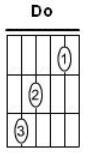
\includegraphics[width=\accordsize]{methodologie/image21.png}
%     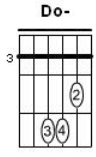
\includegraphics[width=\accordsize]{methodologie/image17.png}
%     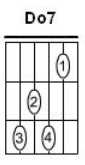
\includegraphics[width=\accordsize]{methodologie/image3.png}
%     \newline
%     \vspace{5cm}
%     % Ré
%     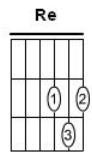
\includegraphics[width=\accordsize]{methodologie/image10.png}
%     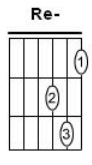
\includegraphics[width=\accordsize]{methodologie/image7.png}
%     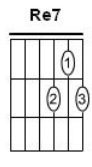
\includegraphics[width=\accordsize]{methodologie/image23.png}
%     \newline
%     \vspace{4pt}
%     % Mi
%     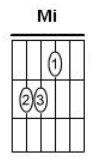
\includegraphics[width=\accordsize]{methodologie/image11.png}
%     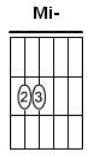
\includegraphics[width=\accordsize]{methodologie/image12.png}
%     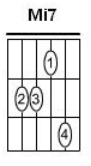
\includegraphics[width=\accordsize]{methodologie/image14.png}
% \end{figure}
% \begin{figure}[h]
%     \centering
%     % Fa
%     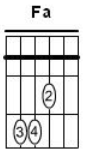
\includegraphics[width=\accordsize]{methodologie/image16.png}
%     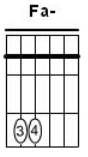
\includegraphics[width=\accordsize]{methodologie/image22.png}
%     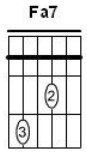
\includegraphics[width=\accordsize]{methodologie/image4.png}
%     \newline
%     \vspace{4pt}
%     % Sol
%     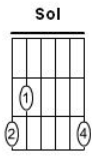
\includegraphics[width=\accordsize]{methodologie/image25.png}
%     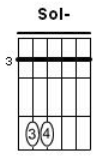
\includegraphics[width=\accordsize]{methodologie/image8.png}
%     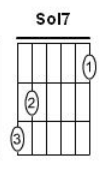
\includegraphics[width=\accordsize]{methodologie/image1.png}
%     \newline
%     \vspace{4pt}
%     % La
%     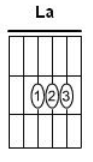
\includegraphics[width=\accordsize]{methodologie/image5.png}
%     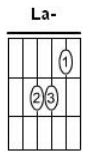
\includegraphics[width=\accordsize]{methodologie/image24.png}
%     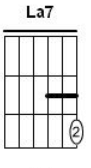
\includegraphics[width=\accordsize]{methodologie/image15.png}
%     \newline
%     \vspace{4pt}
%     % Si
%     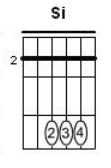
\includegraphics[width=\accordsize]{methodologie/image26.png}
%     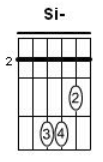
\includegraphics[width=\accordsize]{methodologie/image20.png}
%     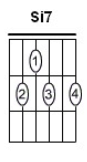
\includegraphics[width=\accordsize]{methodologie/image6.png}
% \end{figure}